\documentclass[a4paper,oneside,11pt]{report}
\usepackage[cm]{fullpage}
\usepackage{lmodern,amsmath,amssymb}
\usepackage{a4wide}
\setlength{\marginparwidth}{3cm}
\setlength{\topmargin}{0cm}
\setlength{\voffset}{0cm}
\setlength{\headsep}{0cm}
\title{ME 603 (FE for Biomechanics) - Lab 1}
\author{Debabrata Auddya}
%\usepackage{etoolbox}
%\preto\equation{\setcounter{equation}{0}}
%\makeatletter
%\pretocmd\start@gather{\setcounter{equation}{0}}{}{}
%\pretocmd\start@align{\setcounter{equation}{0}}{}{}
%\pretocmd\start@multline{\setcounter{equation}{0}}{}{}
%\makeatother
\usepackage{listings}
\usepackage{color}
\usepackage{dsfont}
\usepackage{footmisc}
\usepackage{verbatim}
\usepackage{smartdiagram}
\setlength{\marginparwidth}{0cm}
\setlength{\topmargin}{0cm}
\setlength{\voffset}{0cm}
\setlength{\headsep}{0cm}
\definecolor{dkgreen}{rgb}{0,0.6,0}
\definecolor{gray}{rgb}{0.5,0.5,0.5}
\definecolor{mauve}{rgb}{0.58,0,0.82}
\lstset{frame=tb,
	language=Java,
	aboveskip=3mm,
	belowskip=3mm,
	showstringspaces=false,
	columns=flexible,
	basicstyle={\small\ttfamily},
	numbers=none,
	numberstyle=\tiny\color{gray},
	keywordstyle=\color{blue},
	commentstyle=\color{dkgreen},
	stringstyle=\color{mauve},
	breaklines=true,
	breakatwhitespace=true,
	tabsize=3
}
\begin{document}
\maketitle
\section*{1. What step of the FE pipeline is PreView used for?}
In order to set up a finite element problem and perform computations on it, it is important to clearly define the material, its properties and the corresponding mesh. PreView is an FE Preprocessor that allows the user to create or import meshes, specify the boundary conditions and material properties as well as allow the user to choose from a multitude of analysis that is needed for the next steps in the workflow.  
\section*{2. Describe the different modules:}
1. \textbf{Structural Mechanics}:
Mechanics of strcutures is a domain of study within applied mechanics that investigates the response(behaviour) of structures under mechanics loads such as buckling of column, torsion of shaft, deflection of a thin shell, vibration of bridges etc. Essentially the module provides modeling tools and functionality tailored for analyzing mechanical behavior of solid structures. Using the Structural Mechanics Module, one is able to answer questions concerning, for example, stress and strain levels; deformations, stiffness, and compliance; natural frequencies; response to dynamic loads; and buckling instability, to name a few.\\
2. \textbf{Biphasic analysis}: It is used to model two intrinsically incompressible phases (eg proteoglycan, collagen and interstitial fluid).For instance analysis of a biphasic model can describe a tissue's experimentally observed creep and stress-relaxation responses under various loading configurations. \\
3. \textbf{Multiphasic analysis}: The module which deals with the analysis of materials with different states or phases, or, materials in the same physical state and variable chemical composition. \\
4. \textbf{Heat transfer analysis} : The Heat Transfer module is used to analyze the temperature distribution in static and transient heat transfer processes. The Heat Transfer module can be used to design and analyze many different electrical and mechanical systems. Some features include modeling: Steady-state or transient formulation with arbitrary initial field distribution, nonlinear specific heat and flexible time parameters, heat sources generated by electric power losses etc\\
5. \textbf{Fluid Mechanics Module} : This module provides tools for modeling the cornerstones of fluid flow analysis including incompressible and compressible flow, laminar and turbulent flow, single and multiphase flow, free and porous media flow and flow in open domain and thin film flow. These capabilities are implemented through structured fluid flow interfaces in order to define, solve and analyse time dependent(transient) and steady-state flow problems in 2D and 3D. \\
6. \textbf{Fluid-Structure Interaction Module} : The Fluid-Structure Interaction (FSI) multiphysics interface combines fluid flow with solid mechanics to capture the interaction between the fluid and the solid structure. A Solid Mechanics interface and a Single-Phase Flow interface model the solid and the fluid, respectively. The FSI couplings appear on the boundaries between the fluid and the solid. The Fluid-Structure Interaction interface uses an arbitrary Lagrangian-Eulerian (ALE) method to combine the fluid flow formulated using an Eulerian description and a spatial frame with solid mechanics formulated using a Lagrangian description and a material (reference) frame. \\
7. \textbf{Reaction-diffusion analysis} : This module is used to model diffusion controlled reactions of chemical species over spatial and temporal domains and capture its evolution. 
\section*{3. What do the following shortcuts do:}
1. \textbf{CTRL+B} : Opens up the Boundary Condition Window\\
2. \textbf{CTRL+M} : Opens up the Material Window for specifying material of the part\\
3. \textbf{M} : Show/Hide Mesh Lines of the Part\\
4. \textbf{G} : Show/Hide Grid Lines \\
5. \textbf{CTRL+L} : Option for adding Surface Load \\
6. \textbf{F4} : Curve Editor \\
\section*{4. Create a 2 mm radius by 1 mm high cylinder with a butterfly mesh; take an image with the grid and mesh on.}
\begin{figure}[htb]
	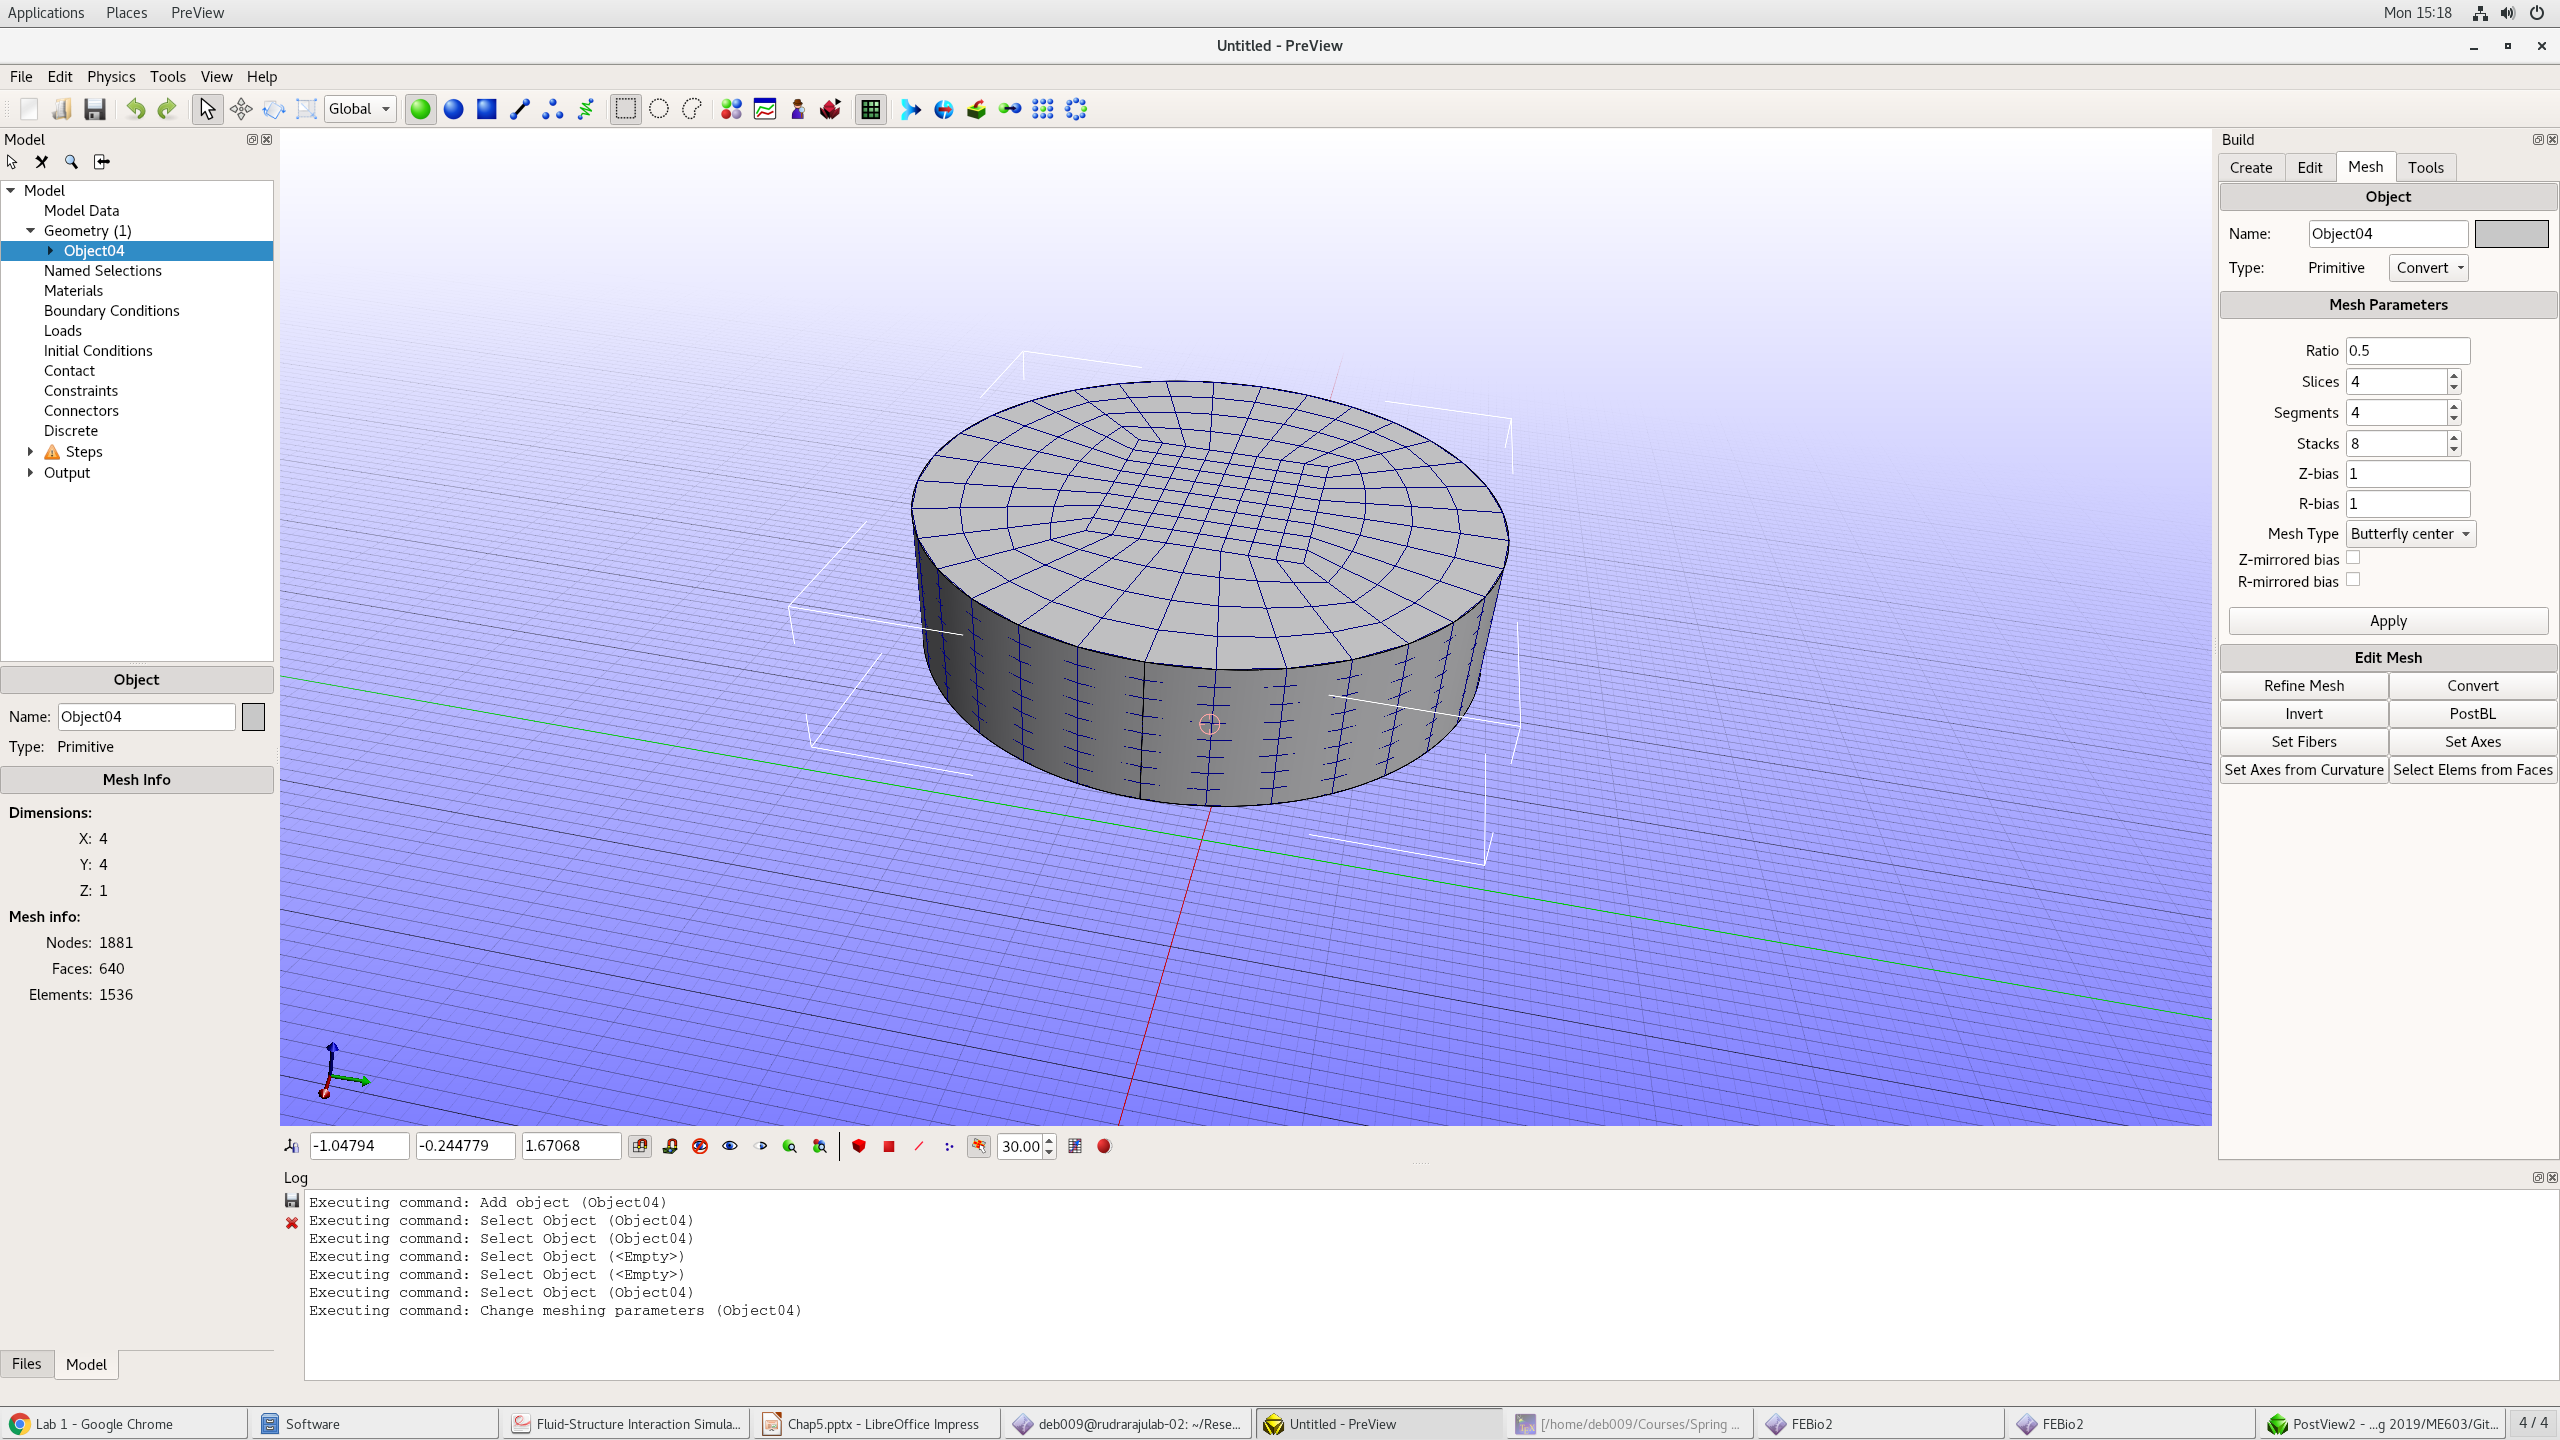
\includegraphics[width=\linewidth]{a0101.png}
	\caption{Butterfly Mesh}
	\label{fig:a0101}
\end{figure}
\textbf{Steps:} \\
1. Create a 2mm radius by 1mm high cylinder \\
2. Make a butterfly mesh \\
%Figure \ref{fig:a0101} shows the model
\section*{5. After completing tutorial 2, take an image of the PreView screen that includes model sections expanded to show the geometry, materials, boundary conditions, and steps.}
\begin{figure}[htb]
	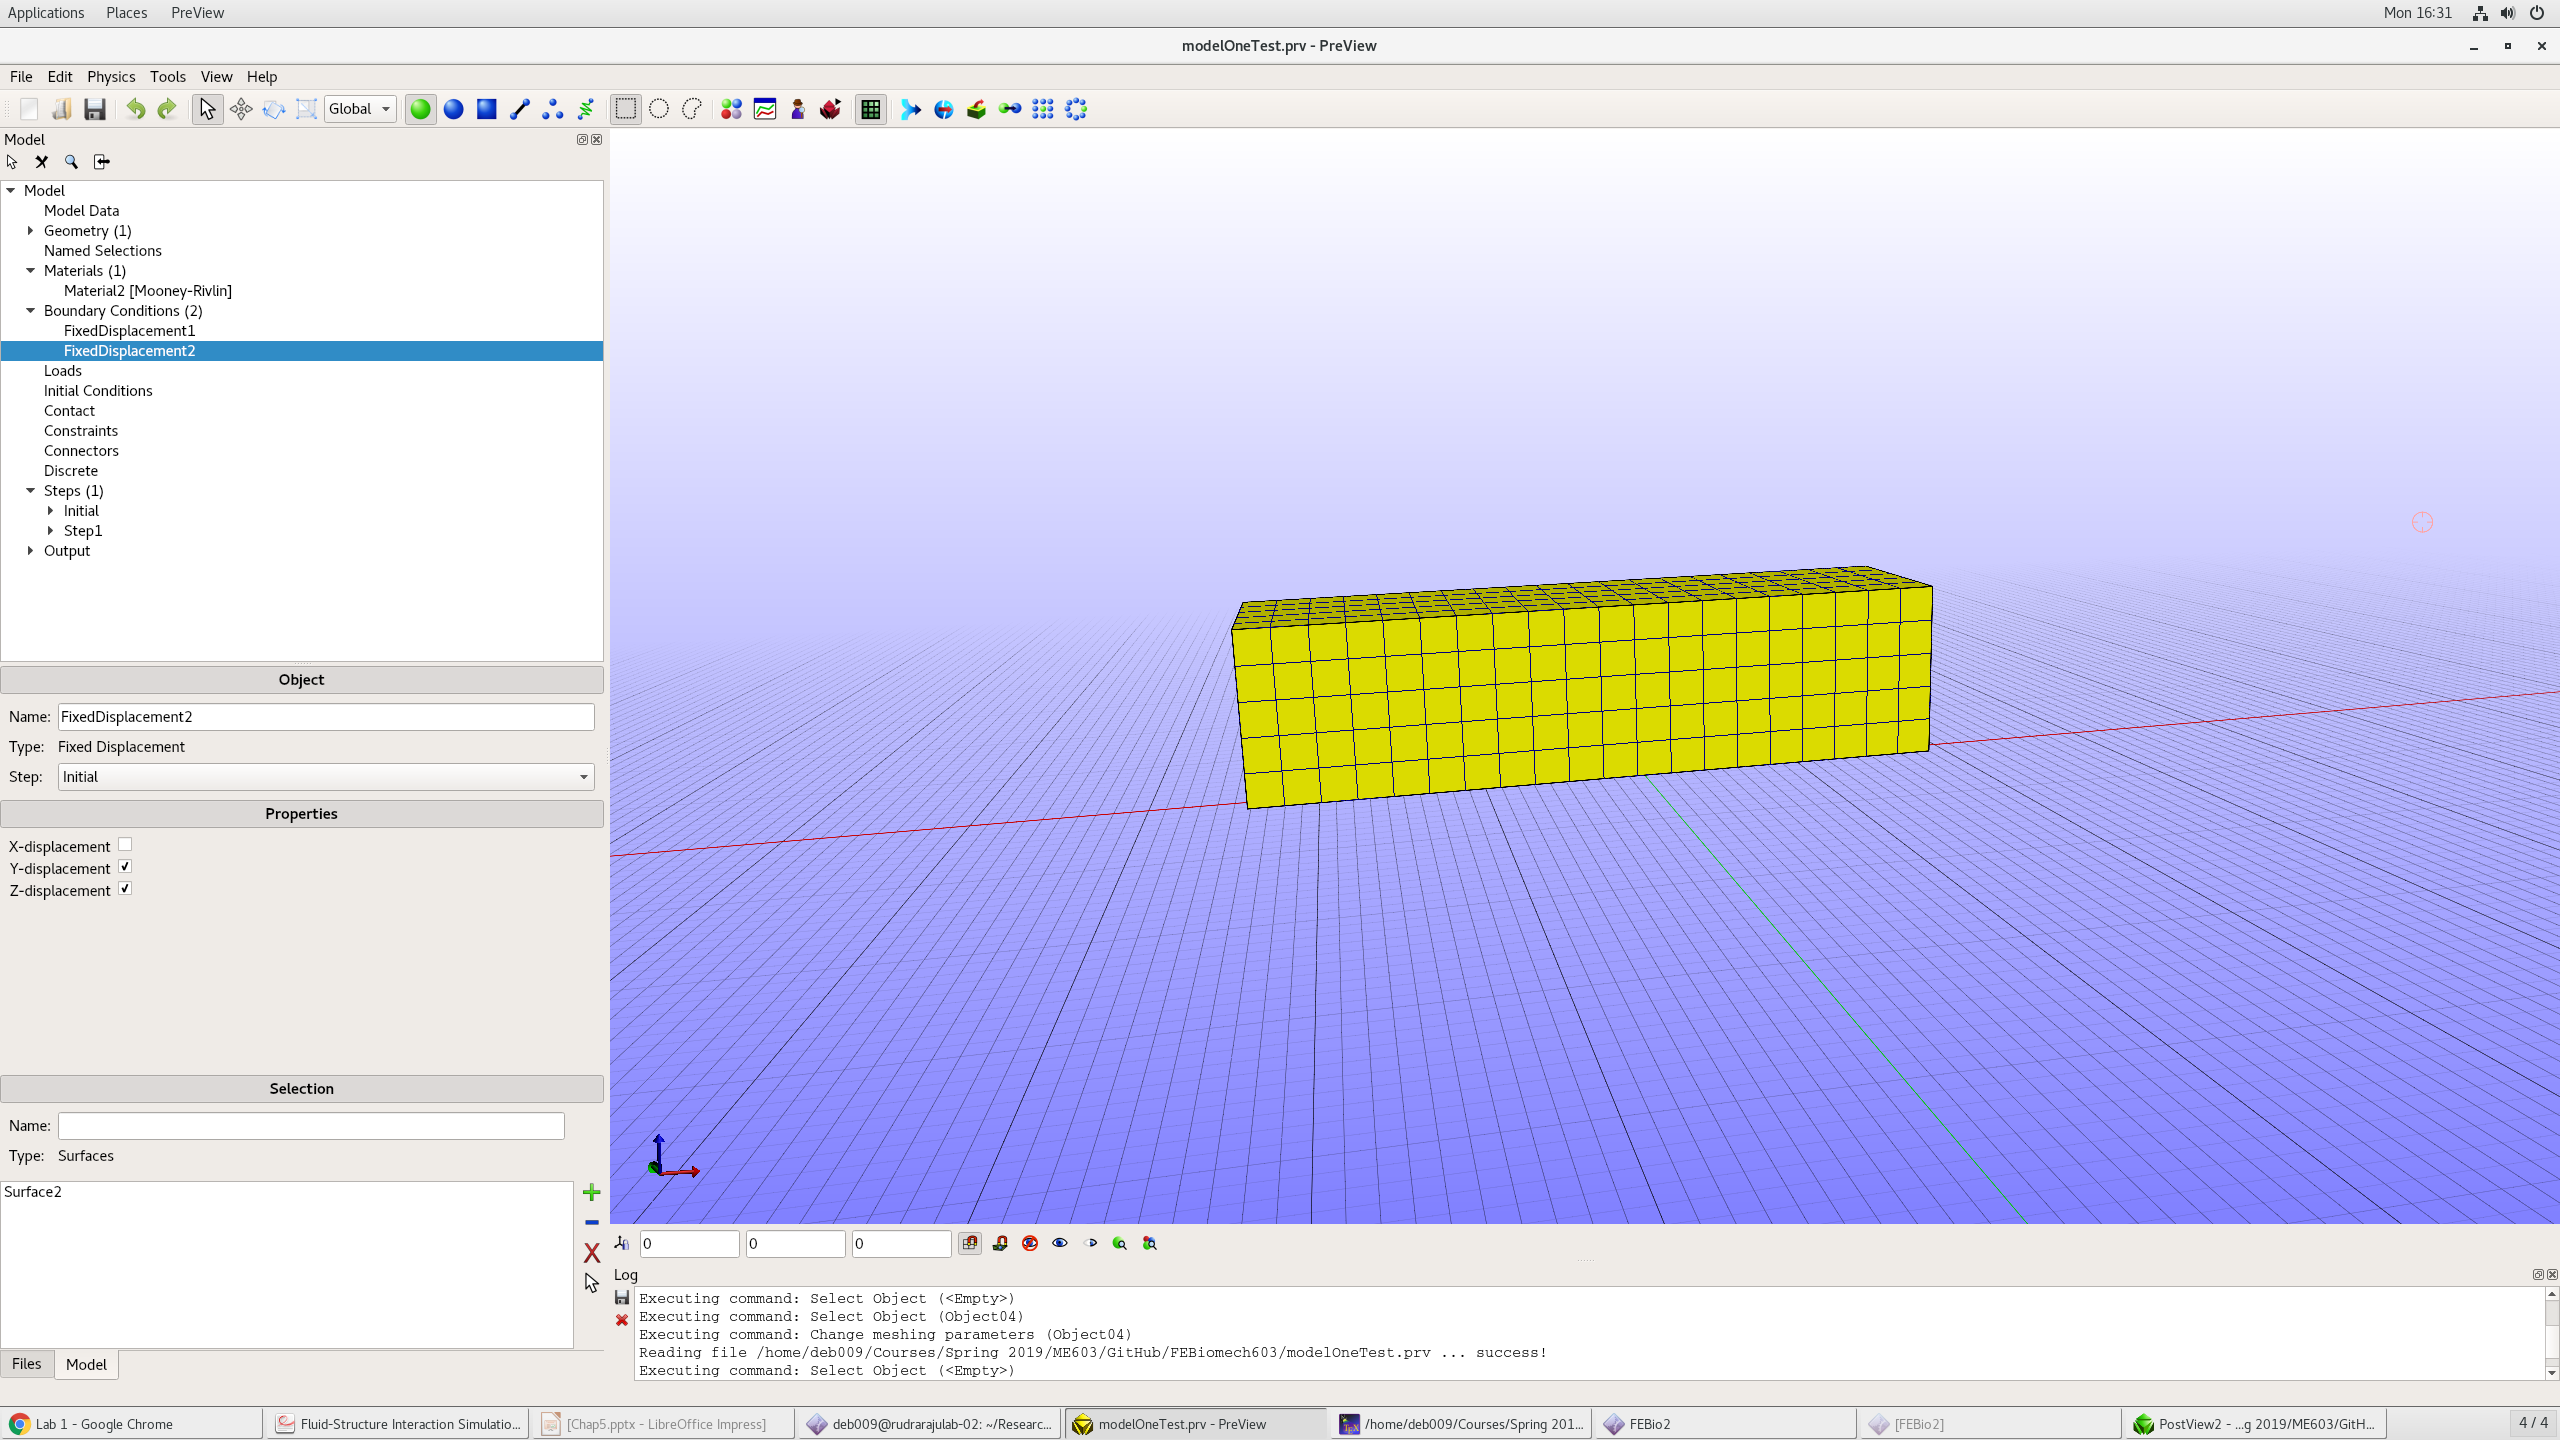
\includegraphics[width=\linewidth]{a0102.png}
	\caption{Preview Screen}
	\label{fig:a0102}
\end{figure}
\section*{6. How much out-of-class time did you spend on this lab?}
About 4.5 hours on the content. 1 hour of editing and proofreading. 
\end{document}
